\section{Common conversion mechanism}[label=sec:conversion-mechanism-key-principles]

\subsection{Key principles}[label=sec:conversion-mechanism-key-principles]

Conversion of building data models and datasets into OWL ontologies and RDF datasets (BIM-to-LD conversion) is usually involves two steps: (i) parsing schema units and data instances to build in-memory objects, and (ii) generating OWL ontologies and RDF datasets from those objects (see \autoref{fig:conversion-process}).
One-step straightforward conversion also can be only used for fixed and very simple data models, where is no object interlinking, for instance, a CSV file with known column types and names.


\begin{figure}
    \centering    
    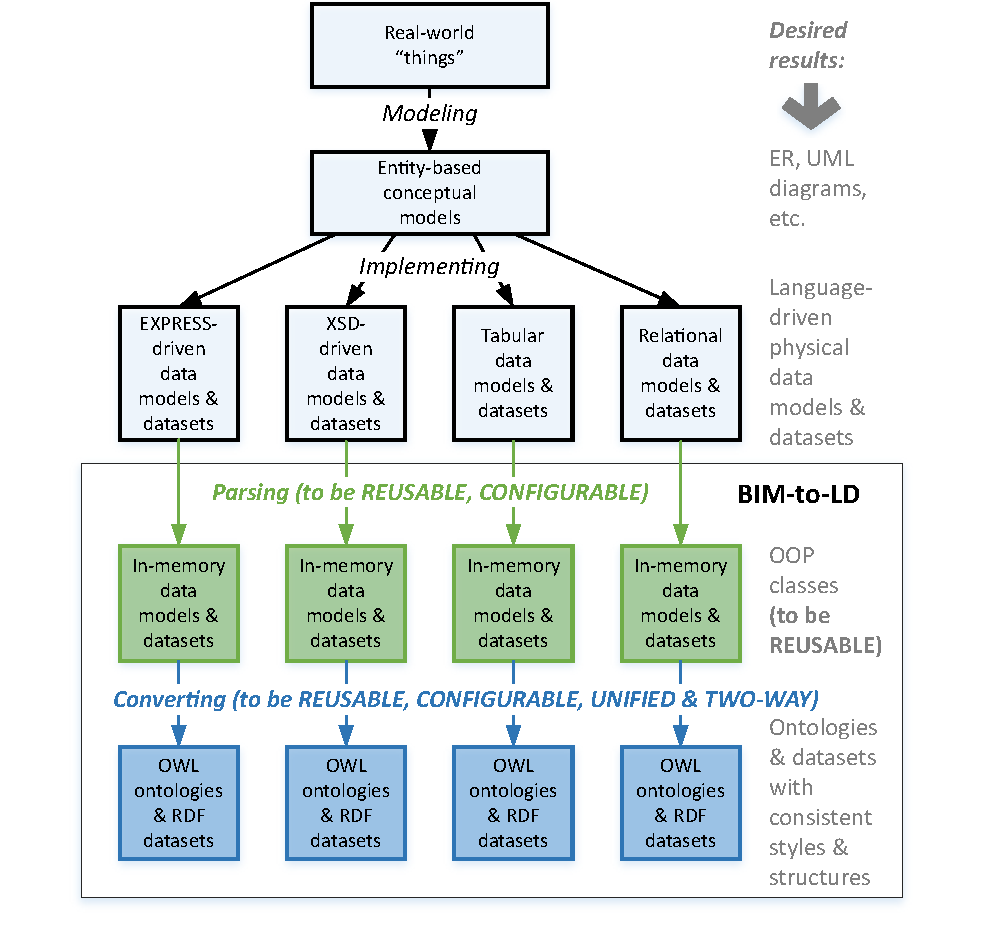
\includegraphics[width=\columnwidth]{images/conversion-process-3.pdf}
    \caption{Two-step BIM-to-LD conversion process}
    \label{fig:conversion-process}
\end{figure}



The main idea of a common BIM-to-LD conversion process via a middle data model is based on requirements of its reusability, flexibility, and consistency.
Reusability allows saving efforts of implementation for each data models and datasets.
Flexibility enables configuration of the whole conversion process as demanded by concrete use cases.
For instance, users will be able to select which OWL 2 profiles generated OWL ontologies and datasets must be conformant to, which data types must be ignored in datasets, whether all data instances must be assigned with URIs and how.
Consistency solves problems ... mentioned in...
It allows ontologies to be aligned with 
to be queries with consitent names/structures... (see paper: Reasoning LD data).
Moreover, consistency between different OWL ontologies is one of important steps to move from "old school" to "new school" of data modeling as proposed by (see \autoref{...}).



The three requested features can be realised mainly thanks to (i) similar characteristics of entity-based data models and (ii) object-oriented programming and design patterns.
As pointed in \autoref{2.1}, data models belonging to one language-driven group has...
However, as will be shown in \autoref{3.2}, 
but also from different groups, 
Thus, it is possible to create an abstract model on top of these data models.
Object design patterns \cite{gamma1995design} provide structural and other patterns to solve common programming problems when both reusability and extensibility are needed.











% (i) reusing parsers and converters for various data models, and (ii) aligning the style and structure of resulting OWL ontologies and RDF datasets.
% As pointed out in \autoref{sec:state-of-the-art}, building data models based on the same schema language have many similarities, so that implementing common parsers and ...  would be rational. 
% Moreover, as will be seen in ..., even between data models from different data model groups there are many comparable properties, so that it is possible to build an abstract object-oriented model based on these features.
% Using a common data model to generate OWL ontologies would result on consistent...

% to keep... consistent as required in...




